\RequirePackage{lineno}
\documentclass[twocolumn,nofootinbib,showpacs,prl,superscriptaddress,secnumarabic,amssymb,nobibnotes,aps,floatfix]{revtex4}
\usepackage{graphicx}
\usepackage{hyperref}
\usepackage{amsmath}
\usepackage{dcolumn}% Align table columns on decimal point
\usepackage{bm}% bold math
%
\def\Dirac#1{#1\hskip-5pt/}
%
\newcommand*\patchAmsMathEnvironmentForLineno[1]{%
\expandafter\let\csname old#1\expandafter\endcsname\csname #1\endcsname
\expandafter\let\csname oldend#1\expandafter\endcsname\csname end#1\endcsname
\renewenvironment{#1}%
{\linenomath\csname old#1\endcsname}%
{\csname oldend#1\endcsname\endlinenomath}}%
\newcommand*\patchBothAmsMathEnvironmentsForLineno[1]{%
\patchAmsMathEnvironmentForLineno{#1}%
\patchAmsMathEnvironmentForLineno{#1*}}%
\AtBeginDocument{%
\patchBothAmsMathEnvironmentsForLineno{equation}%
\patchBothAmsMathEnvironmentsForLineno{align}%
\patchBothAmsMathEnvironmentsForLineno{flalign}%
\patchBothAmsMathEnvironmentsForLineno{alignat}%
\patchBothAmsMathEnvironmentsForLineno{gather}%
\patchBothAmsMathEnvironmentsForLineno{multline}%
}


%
\begin{document}
%\linenumbers

\title{Incoherent Deep Virtual Compton Scattering off $^4$He using CLAS 
spectrometer}

\newcommand*{\ANL}{Argonne National Laboratory, Argonne, Illinois 60439}
\newcommand*{\ANLindex}{1}
\affiliation{\ANL}
\newcommand*{\ORSAY}{Institut de Physique Nucl\'eaire, CNRS/IN2P3 and Universit\'e Paris Sud, Orsay, France}
\newcommand*{\ORSAYindex}{2}
\affiliation{\ORSAY}
\newcommand*{\JLAB}{Thomas Jefferson National Accelerator Facility, Newport News, Virginia 23606}
\newcommand*{\JLABindex}{3}
\affiliation{\JLAB}
 
\newcommand*{\NOWJLAB}{Thomas Jefferson National Accelerator Facility, Newport News, Virginia 23606}
\newcommand*{\NOWODU}{Old Dominion University, Norfolk, Virginia 23529}
 %%%%%%%%%%%%%%% END OF Latex Macros for institute addresses  %%%%%%%%%%%%%%%%%%%%%%%%% 

\author {M.~Hattawy}
\affiliation{\ANL}
\affiliation{\ORSAY}
\author {R.~Dupr\'{e}} 
\affiliation{\ANL}
\affiliation{\ORSAY}
\author {N.A.~Baltzell} 
\affiliation{\ANL}
\affiliation{\JLAB}
\author {K.~Hafidi} 
\email[corresponding author: ]{kawtar@anl.gov}
\affiliation{\ANL}


\collaboration{The CLAS Collaboration}
\noaffiliation

%
\date{\today}
\begin{abstract}
We report the incoherent beam-spin asymmetry measurement of deeply virtual 
Compton scattering (DVCS) off $^4$He. The experiment used the 6 GeV electron 
beam from Jefferson Lab projected onto a $^4$He target in the center of the 
CEBAF Large Acceptance Spectrometer (CLAS).
\end{abstract}
\pacs{Valid PACS appear here}

\maketitle 

The main access to GPDs is through the measurement of deep virtual Compton 
scattering (DVCS), i.e. the hard exclusive electroproduction of a real photon.  
While other processes are known to be sensitive to GPDs, the measurement of
DVCS is considered the cleanest probe and has been the focus of a worldwide effort 
\cite{Stepanyan:2001sm,Airapetian,Chekanov:2003ya,Aktas:2005ty,Chen:2006na,Munoz 
Camacho:2006hx,Girod:2007aa,Mazouz:2007aa,Gavalian:2009,Seder:2015,Pisano:2015,Jo:2015ema}
involving several accelerator facilities such as Jefferson Lab (JLab), HERA and  
CERN. The vast majority of these measurements focused on the study of proton 
structure and allowed extraction of the tomography of the nucleon (for details 
on the formalism, see 
\cite{Goeke:2001tz,Diehl:2003ny,Ji:2004gf,Belitsky:2005qn,Boffi:2007yc,Guidal:2013rya}).

\begin{figure}[tb]
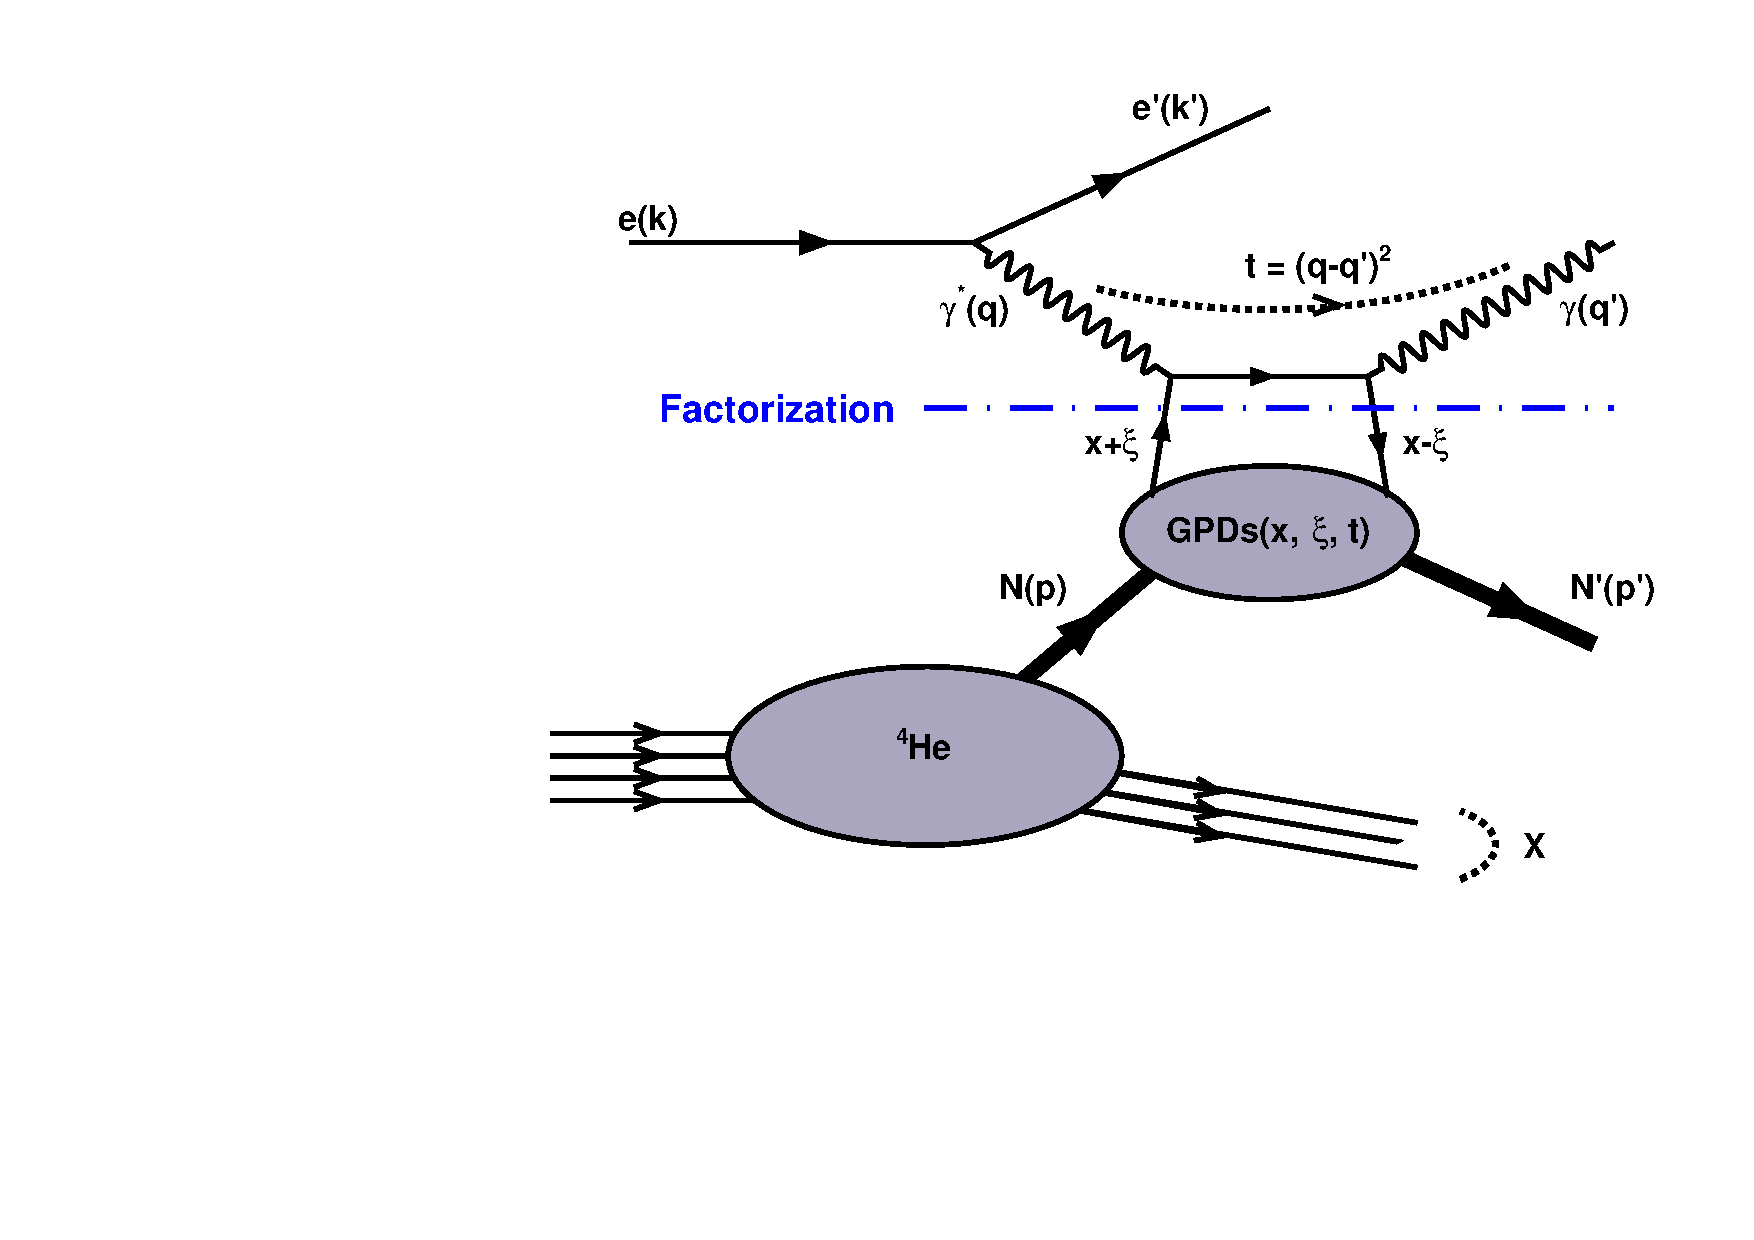
\includegraphics[width=7.5cm]{figs/handbag_incoherent.pdf}
\caption{Representation of the leading-order, twist-2, handbag diagram of the 
incoherent DVCS process off $^4$He.}
\label{fig:diags}
\end{figure}

%experimental setup

The experiment E08-024 took place in Hall-B at JLab
in 2009 using the nearly 100\% duty factor, longitudinally 
polarized electron beam (83$\%$ polarization) at its full energy of 6.064 
GeV. The data were collected over three months using a 6 atm gaseous $^4$He 
target placed in the center of CLAS. For DVCS experiments, the CLAS baseline 
design \cite{Mecking:2003zu} is supplemented with an inner calorimeter (IC) and 
a solenoid. The IC extends the photon detection acceptance of CLAS, which was 
originally from 15$^{\circ}$ to 45$^{\circ}$, to polar angles as low as 
4$^{\circ}$. At these small angles the low-energy M\o{}ller electrons produced 
in the target form a very high rate background that is
suppressed by a 5 Tesla solenoid placed around the target. 

%DVCS selection
To identify incoherent DVCS events, we first select events where one electron, 
one proton, and at least one photon are detected in the final state. Electrons 
are identified by using fiducial cuts and requiring appropriate signals in all 
the sub-detectors of the baseline CLAS (drift chambers, Cherenkov counters, 
electromagnetic calorimeter, and time of flight scintillators). Protons were 
identified with fiducial and timing cuts using the CLAS drift chambers and time 
of flight scintillators. In addition, we apply a vertex matching cut to ensure 
the electron and the proton originate from the same position. The photons are 
detected in either the IC or the CLAS electromagnetic calorimeter.  Note that 
even though the DVCS reaction has only one real photon in the final state, 
events with more than one good photon are not discarded at this stage. This is 
motivated by the fact that, while soft photons are likely to be produced in 
random coincidence, they cannot be mistaken for the large energy DVCS photons 
($>2$ GeV). The most energetic photon is always considered as the DVCS photon 
candidate.

The main background in the measurement of DVCS is incoherent $\pi^{0}$ 
production. Therefore, we remove events where a $\pi^{0}$ can be identified by 
invariant mass reconstruction of two photons. To ensure the interaction occurs 
at the partonic level and the DVCS handbag diagram is dominant, we select 
events with $Q^{2}>1~[GeV^{2}/c^{2}]$. The exclusivity of the events is 
obtained by applying a set of cuts on the following kinematic variables: the 
co-planarity angle ($\Delta \phi$), the missing energy, the missing mass 
squared, the missing transverse momentum, the missing mass squared of the 
$e'^4He'$ system, and the angle ($\theta$) between the measured photon and the 
missing momentum of the $e'^4He'$ system. The cuts are presented in 
Figure~\ref{fig:kin-cuts}, which shows 3$\sigma$ cuts except for the missing.  
After these requirements, we have about 20k events left, and Figure 
\ref{fig:kin-coverage} presents their
kinematic distributions in ($Q^{2}$,$x_{B}$) and ($Q^{2}$,$-t$).

\begin{figure}[tb]
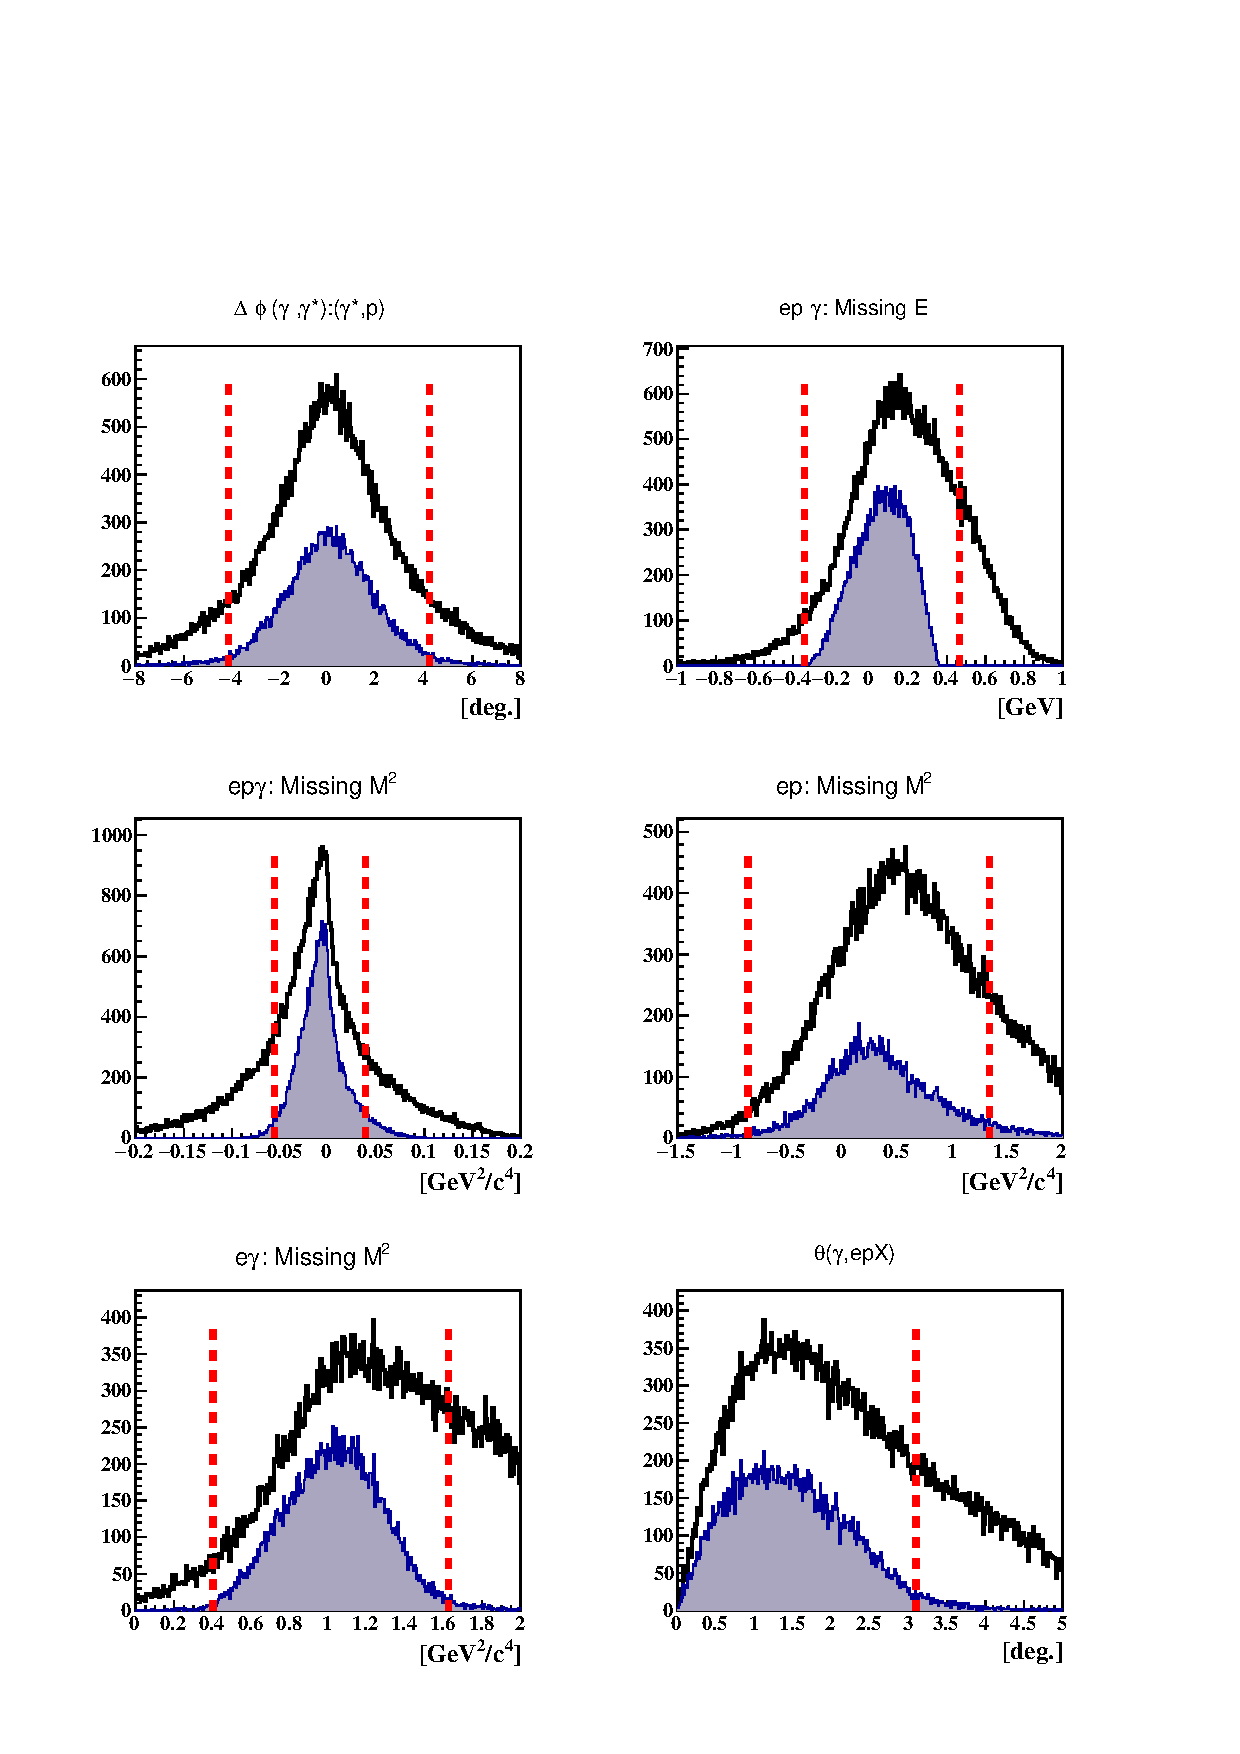
\includegraphics[width=8.9cm]{figs/incoh_exc_cuts_final.pdf}
\caption{The incoherent DVCS exclusivity cuts. The black distributions 
   represent the coherent DVCS events candidate. The shaded distributions 
   represent the events which passed all the exclusivity cuts except the 
   quantity plotted. The vertical red lines represent the applied exclusivity 
cuts. The distributions from left to right and from top to bottoms are: $\Delta 
\phi$, missing energy, missing masses squared and the cone angle ($\theta$) 
between the measured and the calculated photons.}
\label{fig:kin-cuts}
\end{figure}
 

\begin{figure}[tb]
\hspace{-0.45cm}
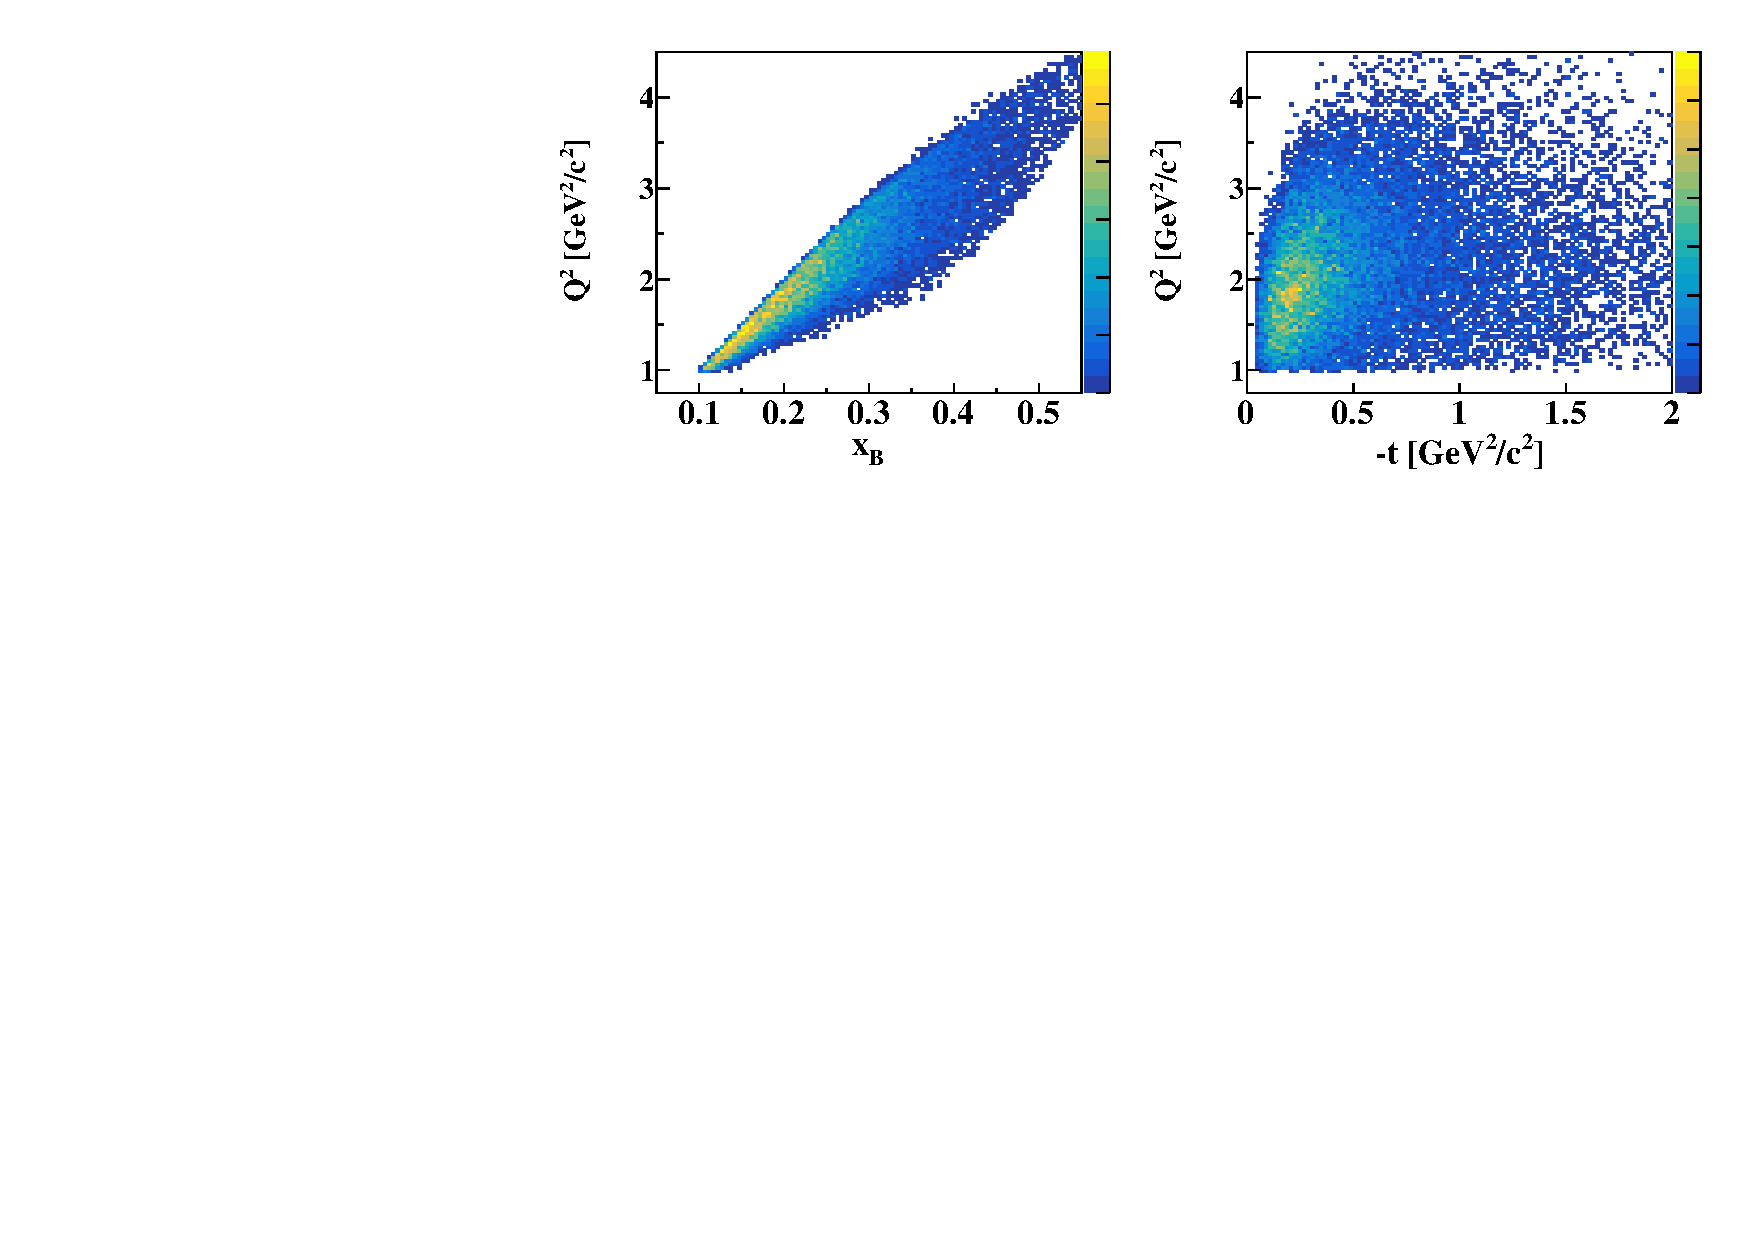
\includegraphics[width=9.0cm]{figs/Q2_xB_t_InCoh.pdf}
\caption{Incoherent DVCS event distributions for $Q^{2}$ as a function of 
$x_{B}$ (left) and $Q^{2}$ as a function of $-t$ (right) after the exclusivity 
cuts.}
\label{fig:kin-coverage}
\end{figure}

%We identified two main backgrounds to our measurement, accidental coincidences 
%and exclusive $\pi^0$ production. The accidental events have particles coming 
%from different events, and we estimate their  contribution
%to be 4.1\% of our sample. We evaluated this contribution by selecting events 
%passing all our cuts but with an electron and an helium originating from 
%different vertices. Regarding the $\pi^0$ production, it can easily be 
%mistaken for DVCS when one of the two photons of the $\pi^0$ decay is produced 
%at low energy in the laboratory frame and remains undetected. To estimate the 
%importance of this background, we developed an event generator calibrated on 
%the experimental yield of exclusive $\pi^0$ measured by our experiment. We 
%used this generator together with a GEANT3 simulation of our detection system 
%to estimate the ratio between
%the number of $\pi^0$ events where the two photons are detected and those that 
%would be mistaken for DVCS. This ratio is then multiplied by the measured 
%yield of exclusive $\pi^0$ events to correct the DVCS data. Depending on the 
%kinematics, we
%found contaminations of 2 to 4\%. The study of systematics errors showed that 
%the main contributions come from the choice of the DVCS exclusivity cuts (8\%) 
%and the large binning size (5.1\%) [Is that right to add it here?]. However, 
%added quadratically, these errors sum up to about 10\%, which always remain 
%significantly smaller than the statistical errors.

%asymmetries
Several observables related to DVCS are of interest, but in this work we focus only 
on the beam-spin asymmetry. This  observable is measurable using a polarized 
lepton beam on an unpolarized target (U). It is convenient to use the beam-spin 
asymmetry because most of the experimental normalization and acceptance issues 
cancel out in the asymmetry ratio. It is defined in terms of the cross sections 
as:
  \begin{equation}
  A_{LU} = \frac{d^{5}\sigma^{+} - d^{5}\sigma^{-} }
                {d^{5}\sigma^{+} + d^{5}\sigma^{-}}.
    \label{BSA_equation}
  \end{equation}
where $d^{5}\sigma^{+(-)}$ is the DVCS differential cross 
section for a positive (negative) beam helicity. Experimentally, $A_{LU}$ 
can be expressed in terms of the measured number of events in each 
beam-helicity state ($N^{+}$, $N^{-}$) as:
\begin{equation}
A_{LU} = \frac{1}{P_{B}} \frac{N^{+} - N^{-}}{N^{+} + N^{-} }.
\end{equation}
where $P_{B}$ is the beam polarization, and $N^{+}$ and $N^{-}$ are the number 
of DVCS events detected with positive and negative electron helicity with 
respect to the beam direction. 

To interpret DVCS, one has to keep in mind that this reaction is 
indistinguishable from the Bethe-Heitler (BH) process, where the final photon 
is emitted either from the incoming or the outgoing leptons. At leading twist 
and leading order, the deeply virtual photon production cross section is 
composed of BH, DVCS, and interference terms. The amplitudes of the 
three terms can be approximated as a finite sum of Fourier harmonics, as shown 
for the nucleon in \cite{Belitsky:2001ns}. 

Due to limited statistics, we only bin  our data two-dimensionally 
 in the azimuthal angle ($\phi$) and one of the kinemtical variables 
$Q^{2}$, $x_{B}$ and $t$. Figure \ref{fig:alu} presents $A_{LU}$ for the three
sets of binning. The asymmetries are fitted with the form of $\frac{\alpha 
sin(\phi)}{1+ \beta cos(\phi)}$.  Figure \ref{fig:alu90} shows the $Q^2$, 
$x_{B}$, and $-t$-dependencies of the fitted $A_{LU}$ signals at 
$\phi$~=~90$^{\circ}$. The $x_{B}$ and $-t$-dependencies are compared to 
theoretical calculations performed by S.~Liuti and K.~Taneja 
\cite{simonetta_2}. Their model relies on the impulse approximation and uses 
advanced spectral functions of nuclei.  The calculations are at slightly 
different kinematics than our data but still provide some guidance. The 
experimental results appear to have larger asymmetries than the calculations.  
These differences may arise from nuclear effects which are not taken into 
account in the model, such as long-range interactions.

\begin{figure}[tb]
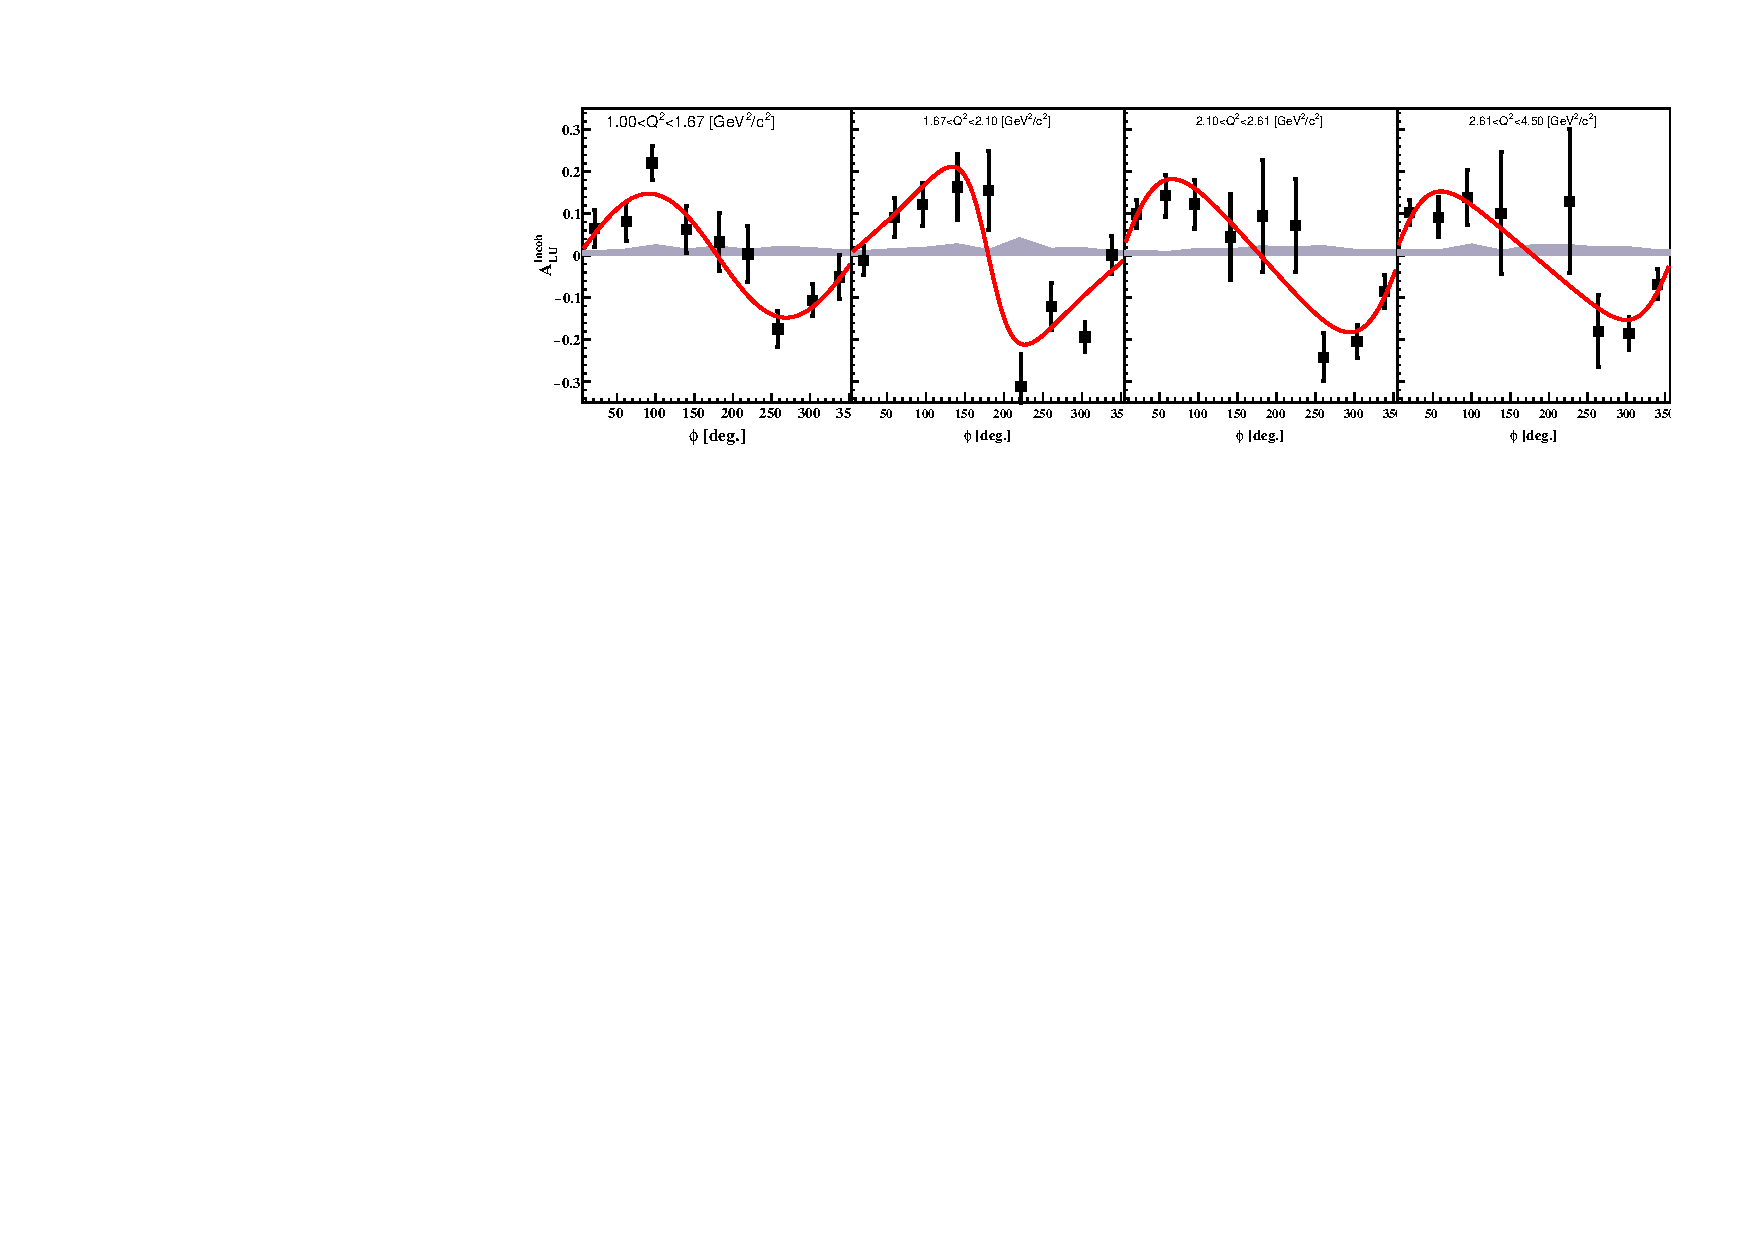
\includegraphics[width=8.9cm]{figs/ALU_phi_p_Q2.pdf}
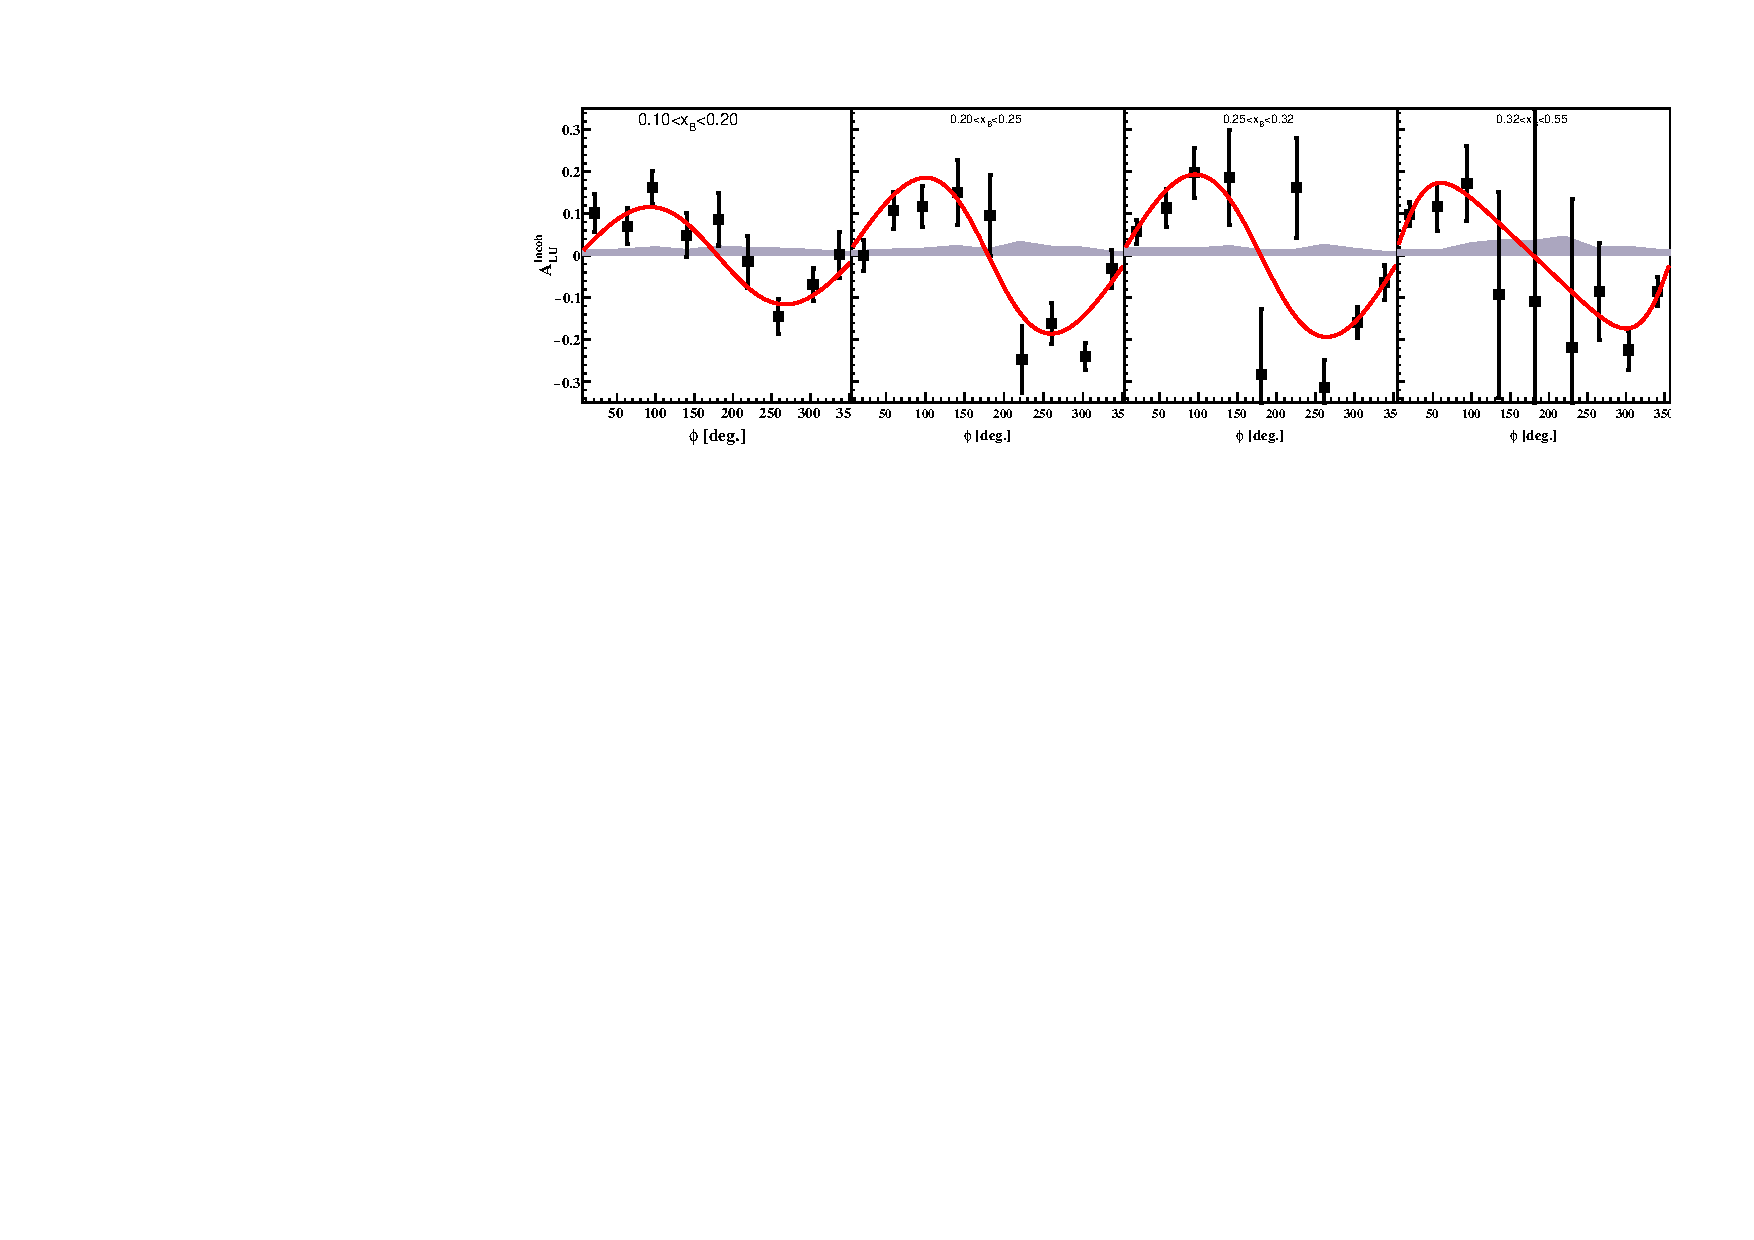
\includegraphics[width=8.9cm]{figs/ALU_phi_p_x.pdf}
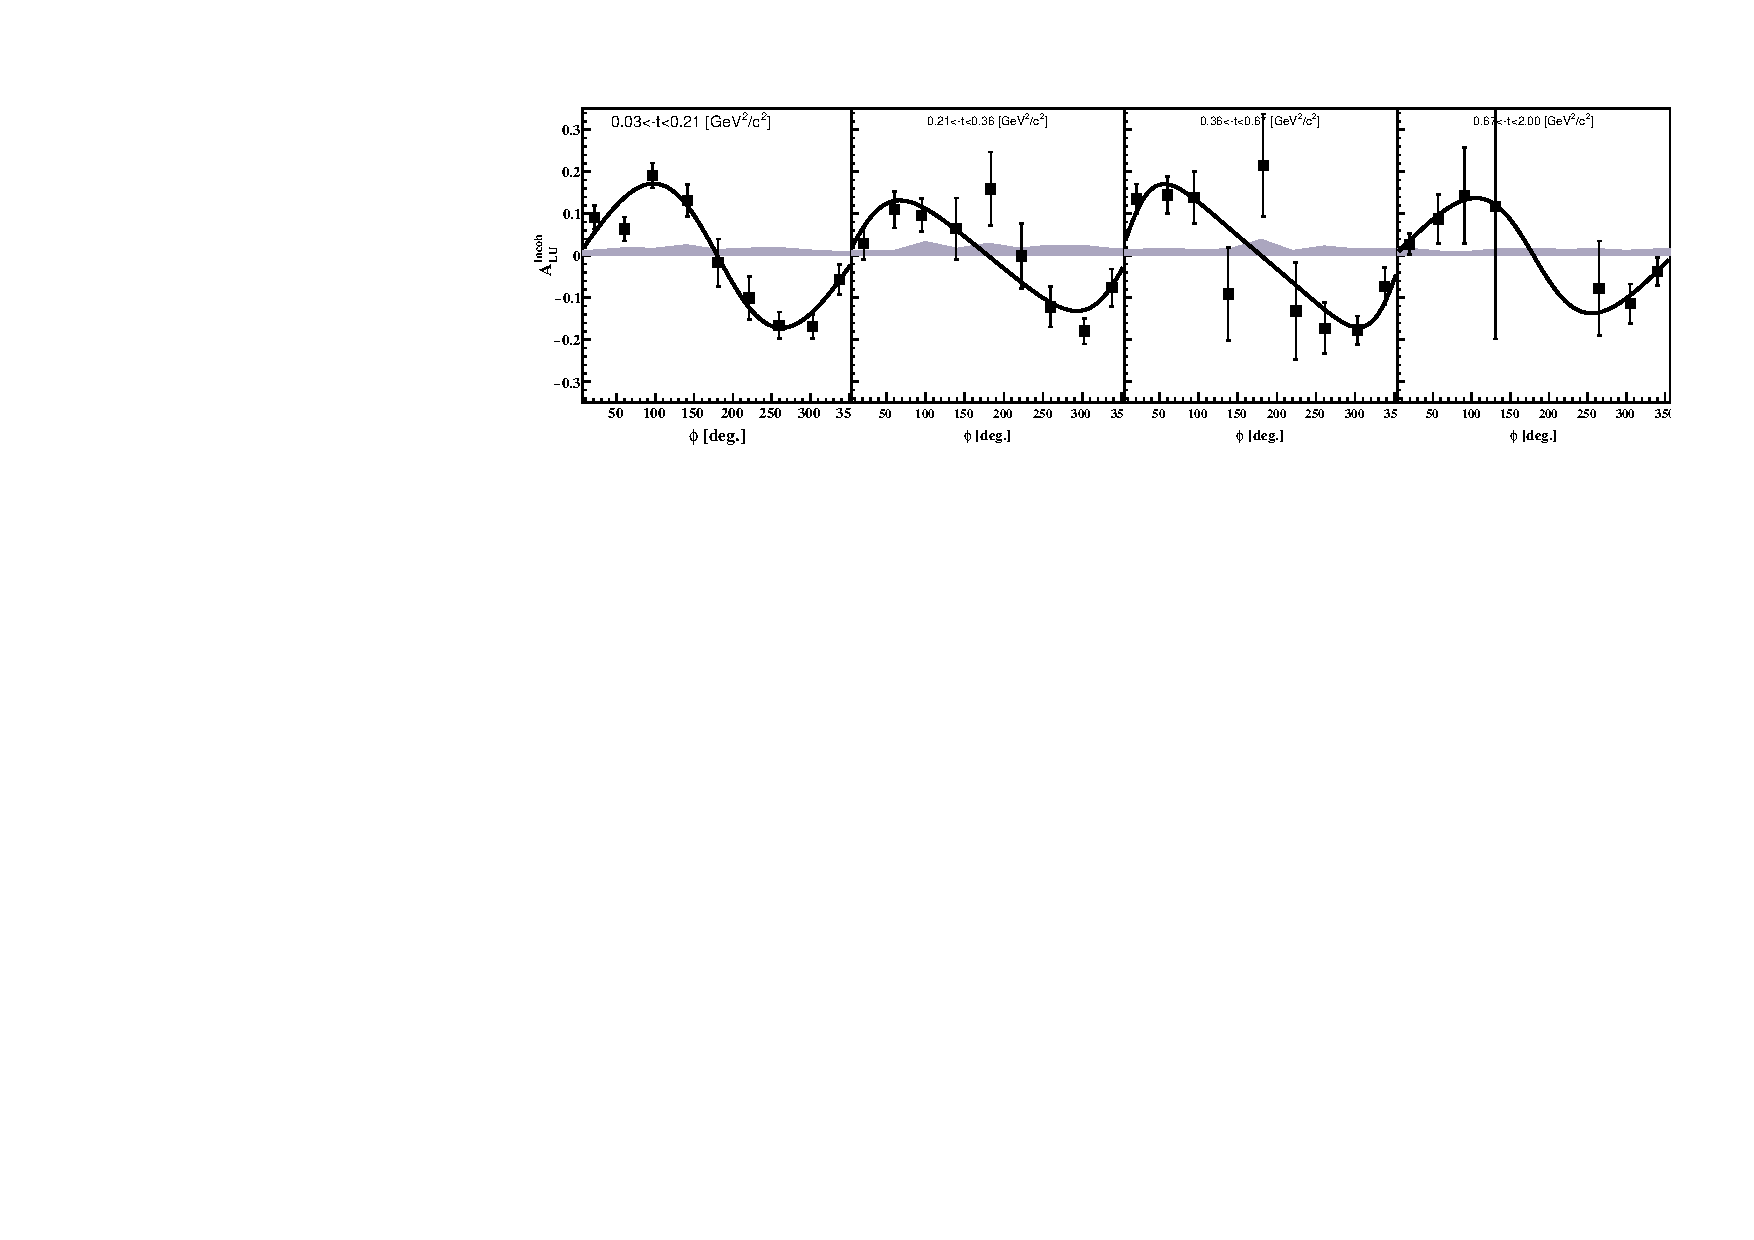
\includegraphics[width=8.9cm]{figs/ALU_phi_p_t.pdf}
\caption{The incoherent $A_{LU}$ as a function of $\phi$. Results are presented
   for different $Q^{2}$ bins (top panel), $x_{B}$ bins (middle panel), and 
   $-t$ bins (bottom panel).  The error bars represent the statistical 
uncertainties. The gray bands represent the systematic uncertainties, including 
the normalisation uncertainties. The red curves are the results of our fits 
with the form $\frac{\alpha sin(\phi)}{1+ \beta cos(\phi)}$.}
\label{fig:alu}
\end{figure}

\begin{figure}[tb]
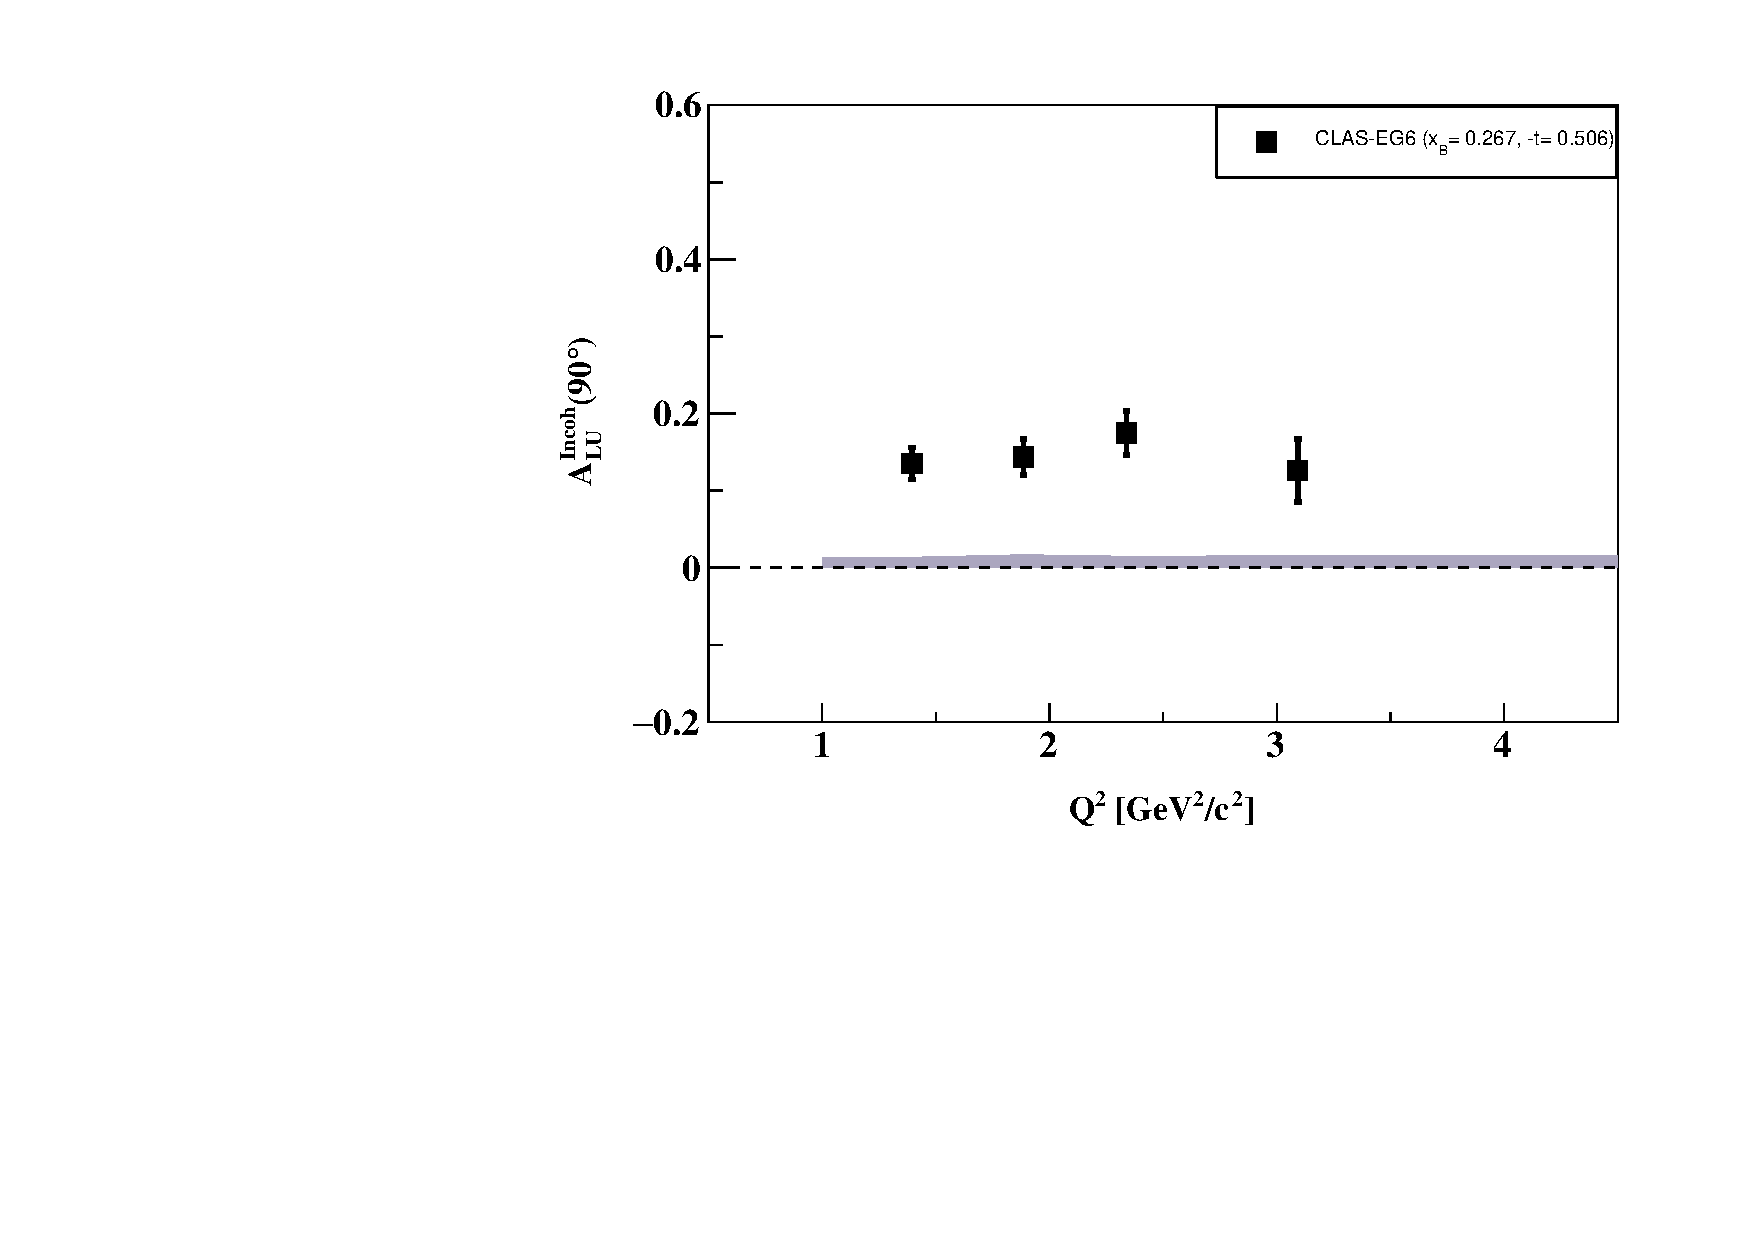
\includegraphics[width=6.9cm]{figs/ALU_90_p_vs_Q2_shortscenrario.pdf}
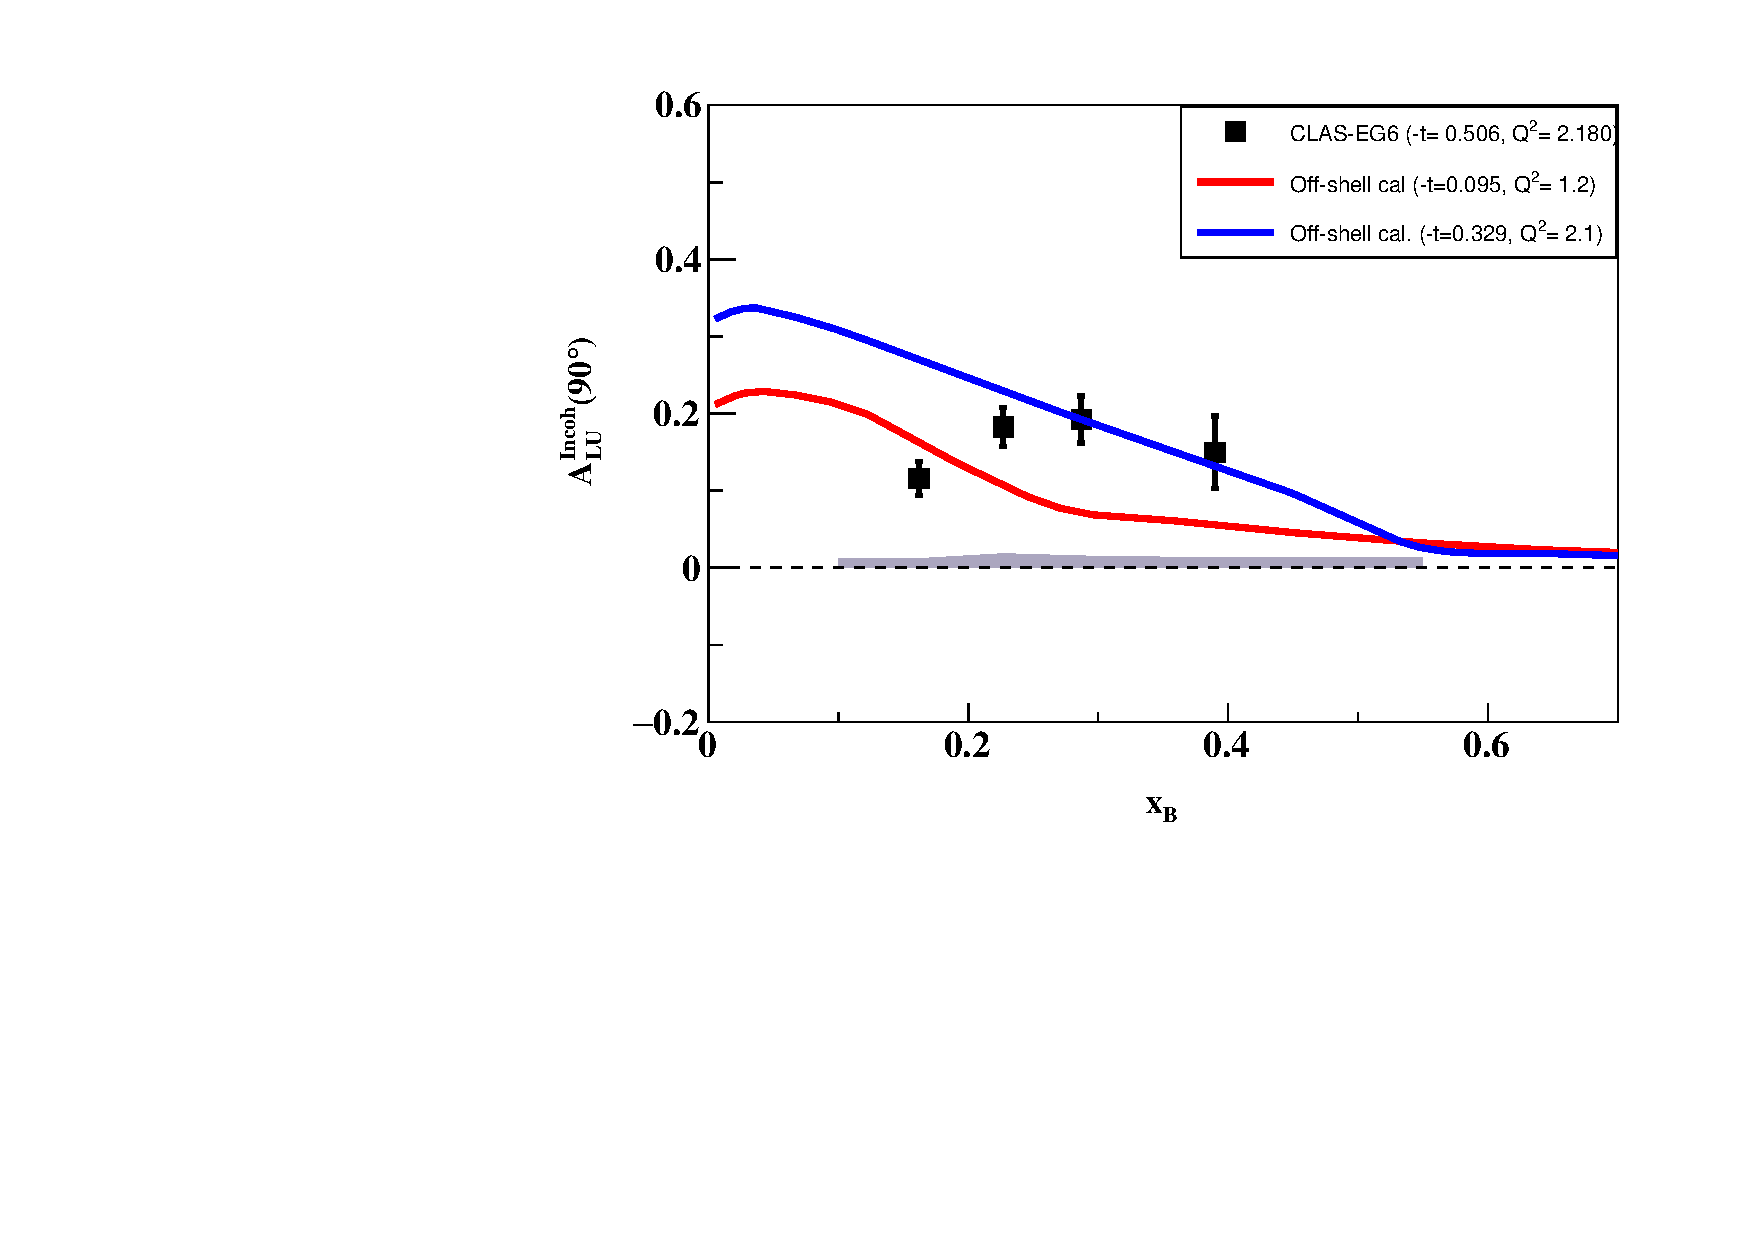
\includegraphics[width=6.9cm]{figs/ALU_90_p_vs_x_shortscenrario.pdf}
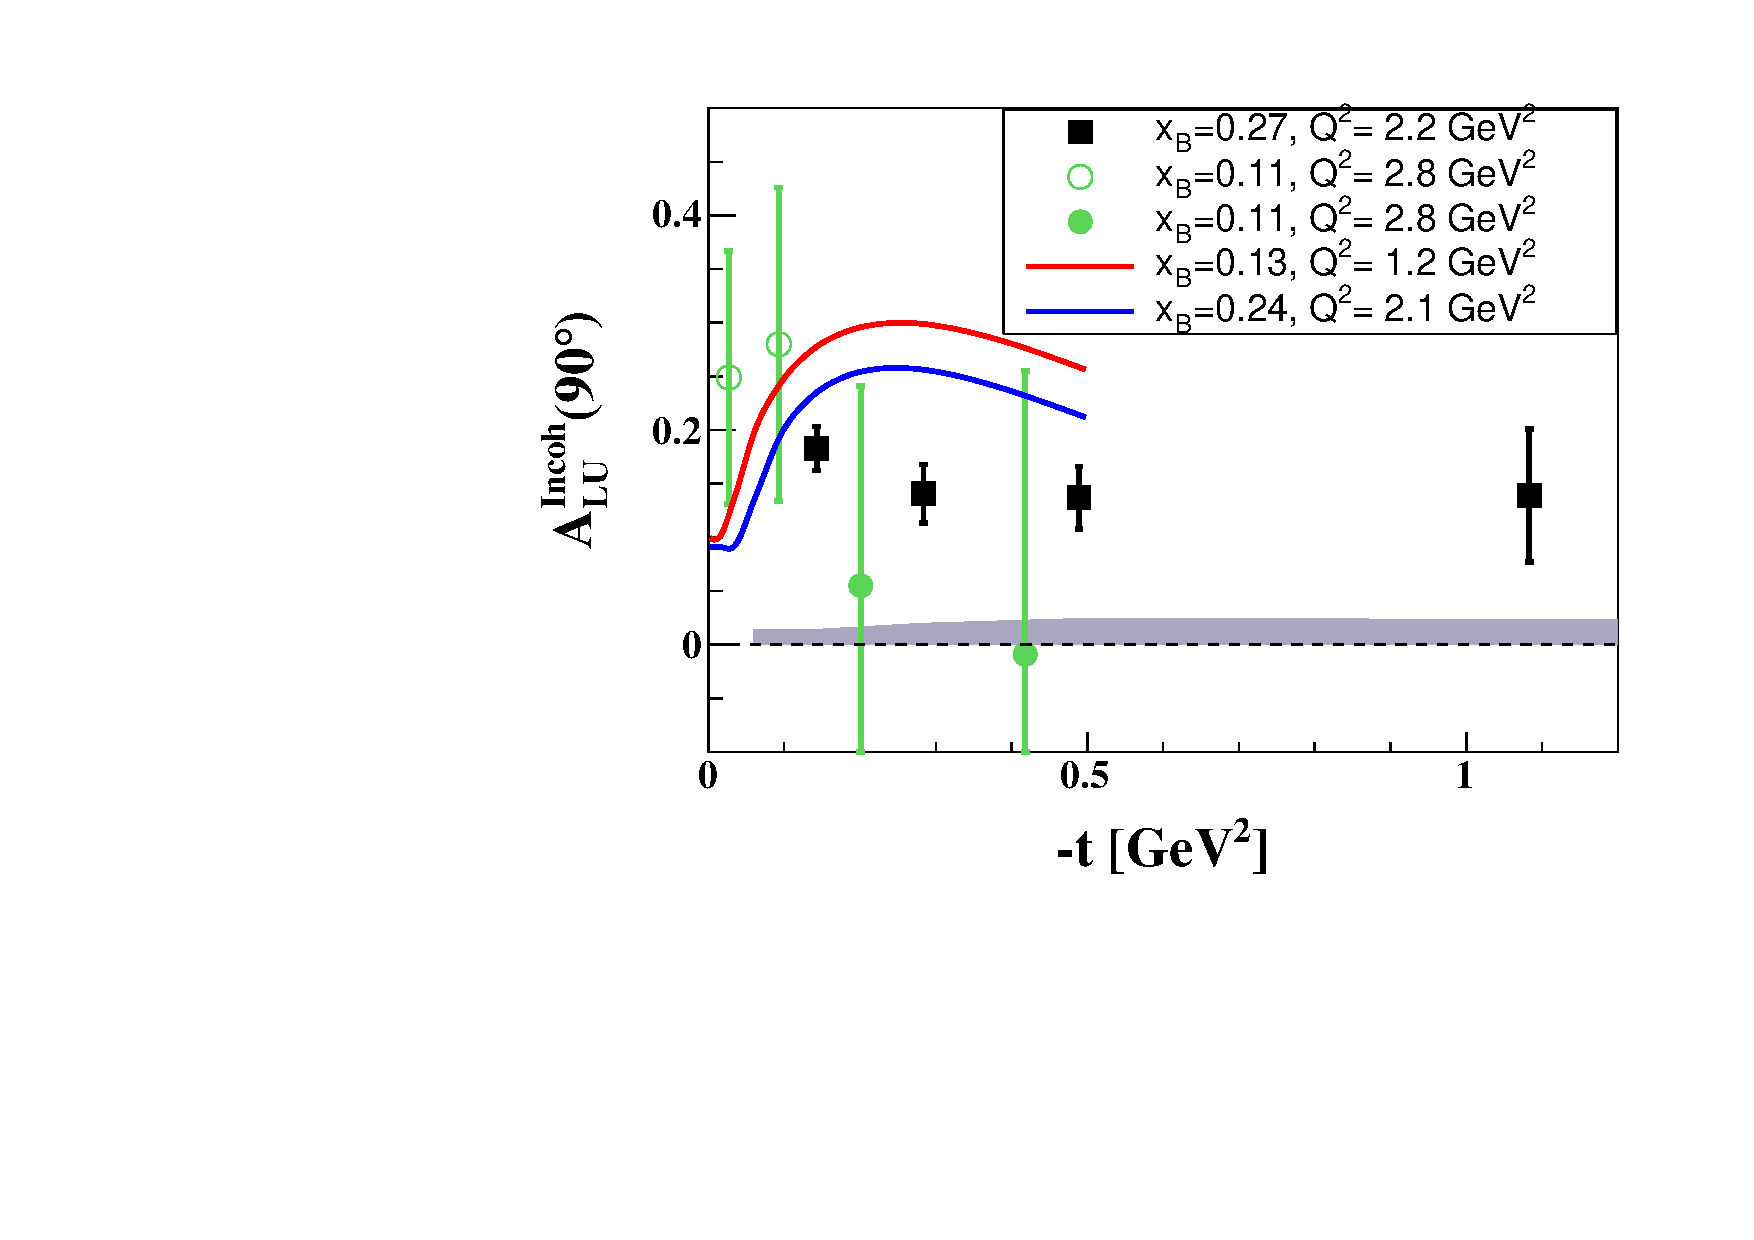
\includegraphics[width=6.9cm]{figs/ALU_90_p_vs_t_shortscenrario.pdf}
\caption{The $Q^{2}$ (left), $x_{B}$ (middle), and $-t$-dependencies (right) of
   the $A_{LU}$ at $\phi$~=~90$^{\circ}$ (black squares). On the 
   middle plot: the full-red and the dashed-blue curves are theoretical 
   calculations from \cite{simonetta_2}. On the right: the green circles are 
   the HERMES $-A_{LU}$ (positron beam was used) inclusive measurements 
\cite{Airapetian}, the colored curves represent theoretical calculations from 
\cite{simonetta_2}.}
\label{fig:alu90}
\end{figure}

\begin{figure}[tp]
\centering
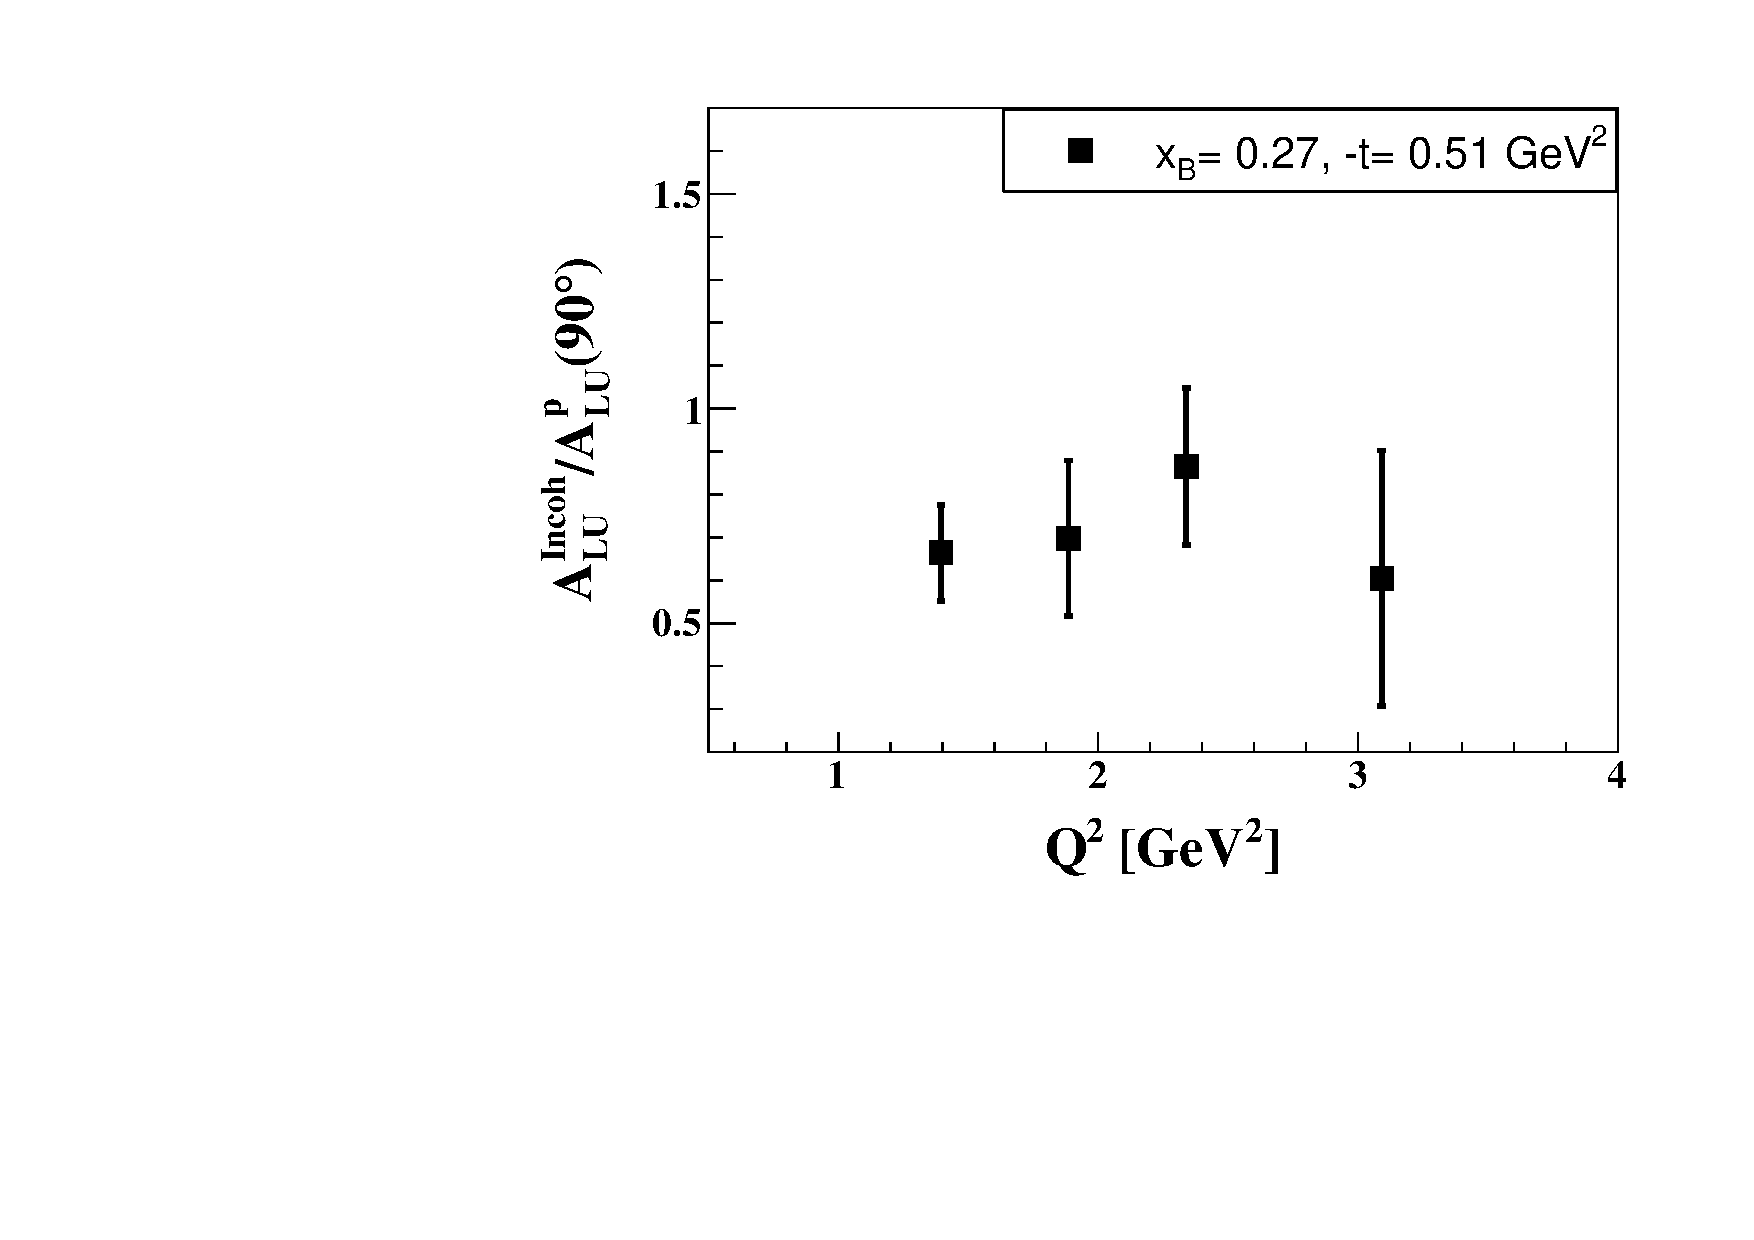
\includegraphics[width=6.9cm]{figs/ALU_ratioInc_Q2_shortscenrario.pdf}\\
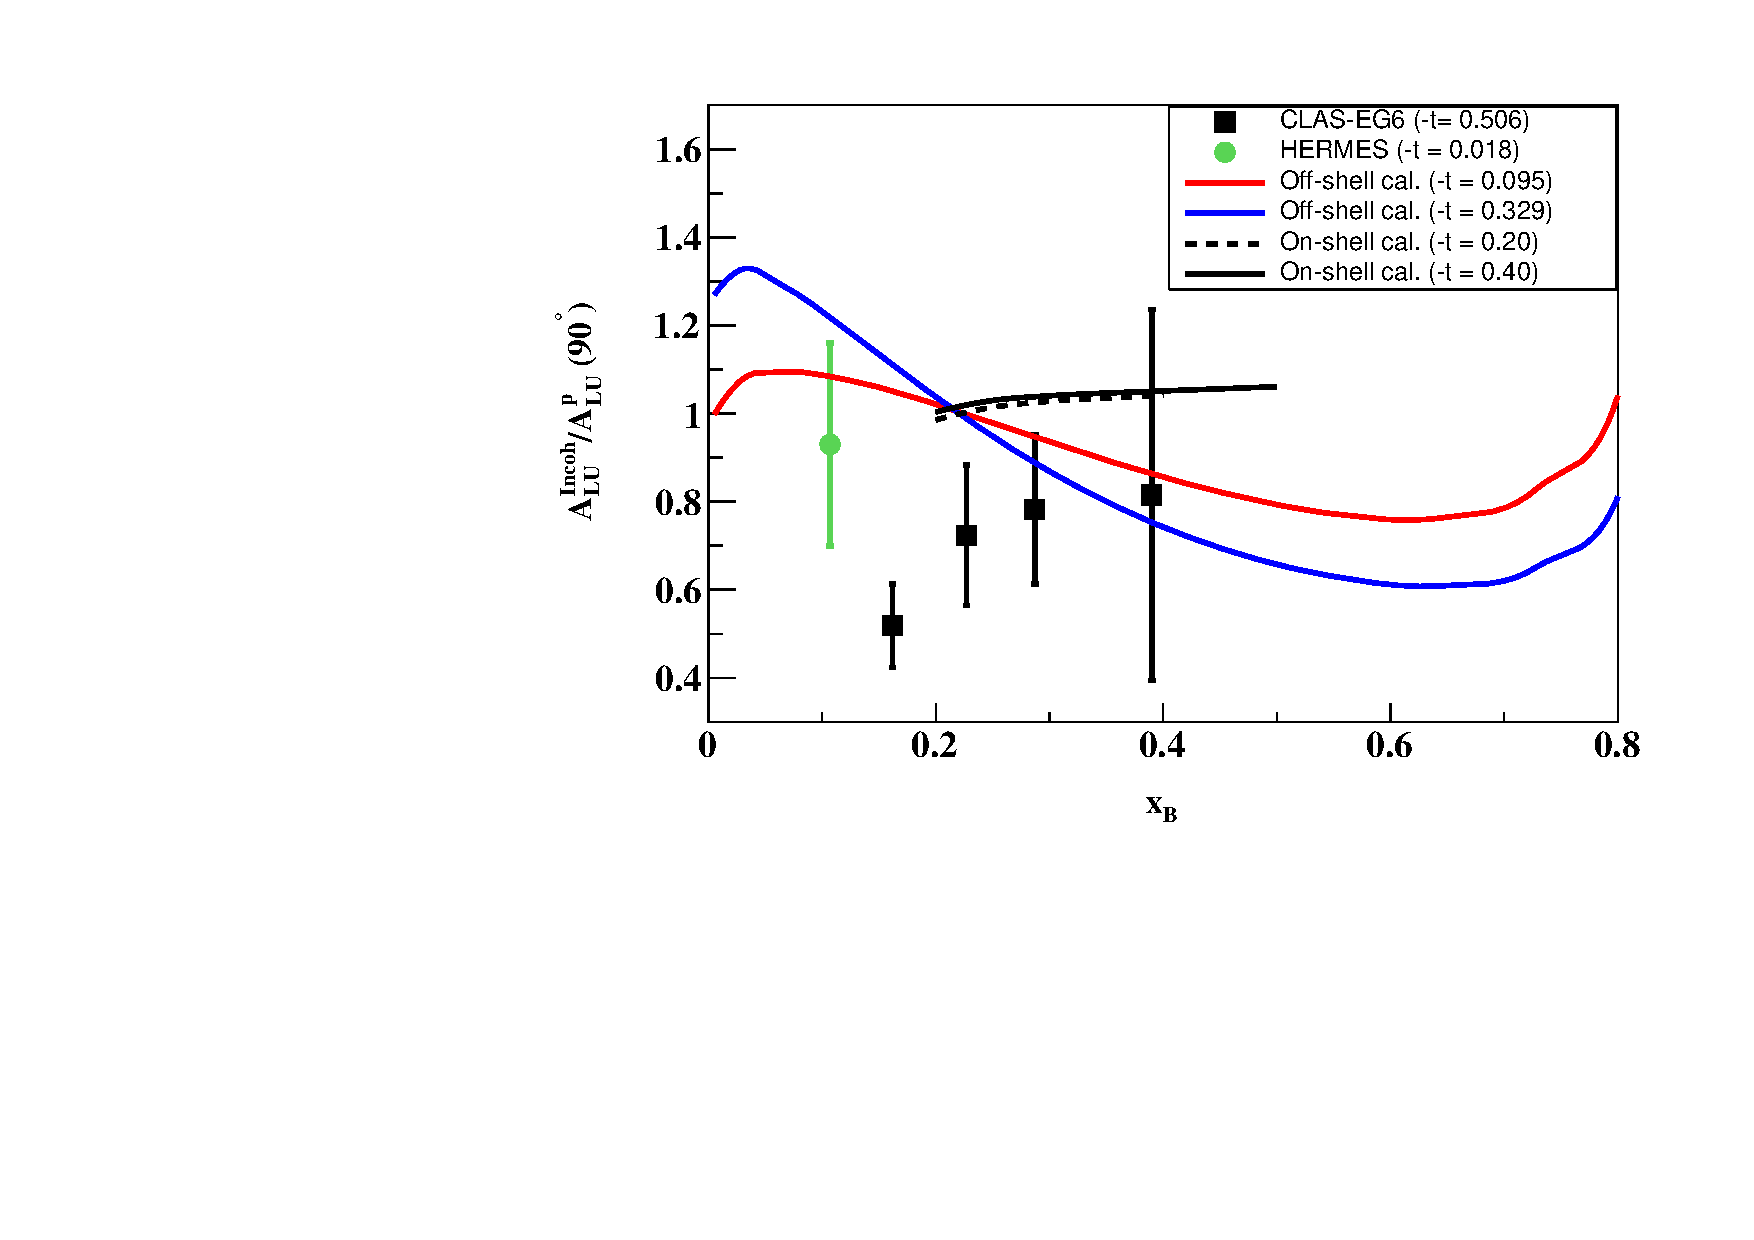
\includegraphics[width=6.9cm]{figs/ALU_ratioInc_x_shortscenrario.pdf}\\
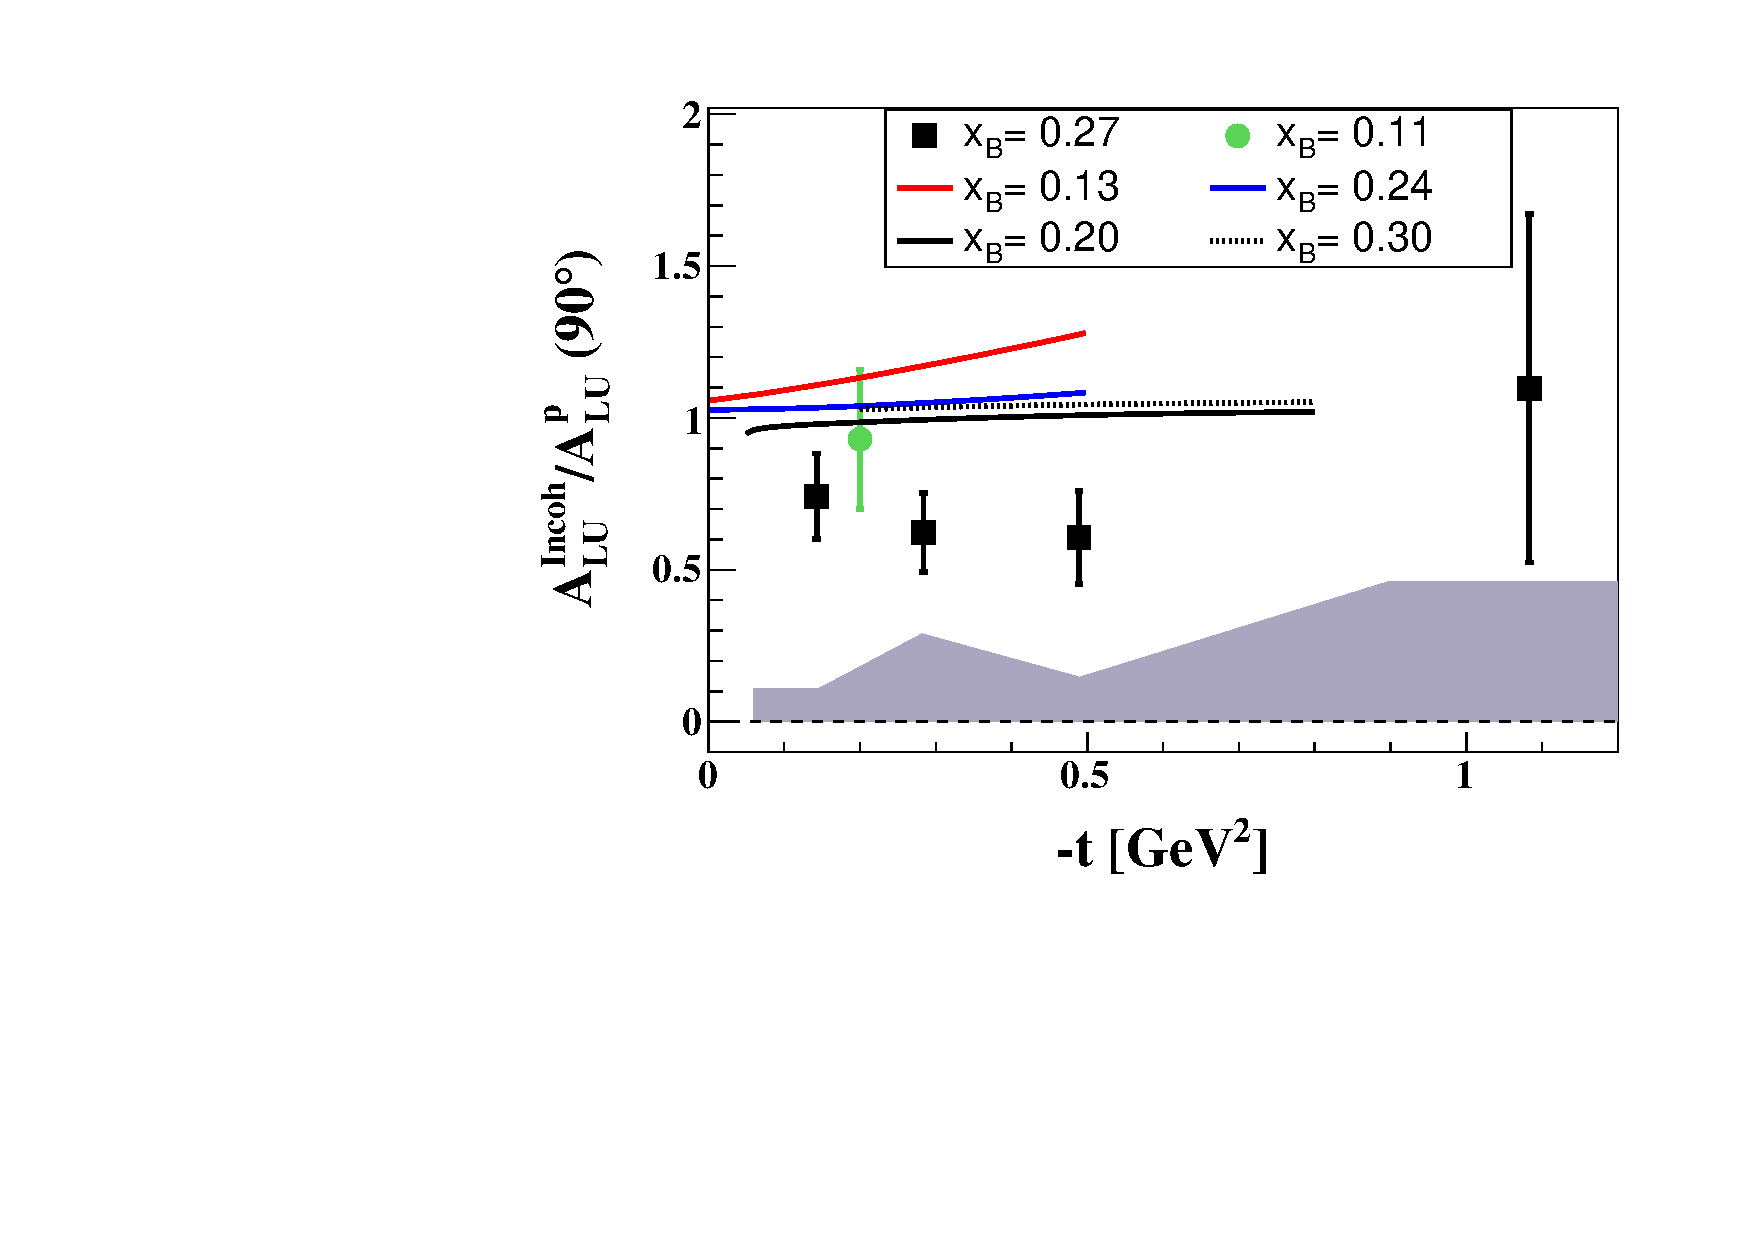
\includegraphics[width=6.9cm]{figs/ALU_ratioInc_t_shortscenrario.pdf}
\caption{ The $A_{LU}$ ratio between the bound and the free proton at 
   $\phi$~=~90$^{\circ}$, as a function of $Q^2$ (on the top), $x_B$ (on the 
   middle), and $t$ (on the bottom). The black squares are our results, the 
   green circles are the HERMES inclusive measurement \cite{Airapetian} 
   results.  The blue and red curves are from an on-shell calculations from S.  
   Liuti and K.  Taneja \cite{simonetta_2}. The solid and dashed black curves 
are from the off-shell calculations \cite{Guzey:2008fe}.} 
\label{fig:incoh_EMC_ratio_ALU_proton}
\end{figure}



%conclusion


%Acknowledgments

We acknowledge the staff of the Accelerator and Physics Divisions at Jefferson 
Lab for making this experiment possible. This work is supported by the U.S.  
Department of Energy, Office of Science, Office of Nuclear Physics contract 
DE-AC05-06OR23177.

\begin{thebibliography}{99}
\bibitem{Mueller:1998fv} 
D. Mueller, D. Robaschik, B. Geyer, F.M. Dittes and J. Horejsi,
Fortsch.\ Phys. {\bf 42}, 101 (1994).
  
\bibitem{Ji:1996ek} 
X.D. Ji,
Phys.\ Rev.\ Lett. {\bf 78}, 610 (1997).

\bibitem{Ji:1996nm} 
X.D. Ji,
Phys.\ Rev.\ D {\bf 55}, 7114 (1997).

\bibitem{Radyushkin:1996nd}
A.V. Radyushkin,
Phys.\ Lett.\  B {\bf 380}, 417 (1996).

\bibitem{Radyushkin:1997ki} 
A.V. Radyushkin,
Phys.\ Rev.\ D {\bf 56}, 5524 (1997).

\bibitem{Burkardt:2000za} 
  M.~Burkardt,
  Phys.\ Rev.\ D {\bf 62}, 071503 (2000)
  Erratum: Phys.\ Rev.\ D {\bf 66}, 119903 (2002)

\bibitem{Diehl:2002he} 
  M.~Diehl,
  Eur.\ Phys.\ J.\ C {\bf 25}, 223 (2002)
  Erratum: Eur.\ Phys.\ J.\ C {\bf 31}, 277 (2003)
 
\bibitem{Belitsky:2002ep} 
  A.~V.~Belitsky and D.~Mueller,
  Nucl.\ Phys.\ A {\bf 711}, 118 (2002)

\bibitem{Burkardt:2005hp} 
  M.~Burkardt,
  Phys.\ Rev.\ D {\bf 72}, 094020 (2005)

\bibitem{Stepanyan:2001sm}
S.~Stepanyan {\it et al.} [CLAS Collaboration],
Phys.\ Rev.\ Lett. {\bf 87}, 182002 (2001).

\bibitem{Airapetian}
A. Airapetian {\it et al.} [HERMES Collaboration],
Phys.\ Rev.\ Lett. {\bf 87}, 182001 (2001);
JHEP {\bf 1207}, 032 (2012);
JHEP {\bf 1006}, 019 (2010);
JHEP {\bf 0806}, 066 (2008);
Phys.\ Lett.\ B {\bf 704}, 15 (2011);
Phys.\ Rev.\  D {\bf 75}, 011103 (2007);
JHEP {\bf 0911}, 083 (2009);
Phys.\ Rev.\ C {\bf 81}, 035202 (2010);
JHEP {\bf 1210}, 042 (2012).

\bibitem{Chekanov:2003ya}
S. Chekanov {\it et al.} [ZEUS Collaboration],
Phys.\ Lett.\  B {\bf 573}, 46 (2003).

\bibitem{Aktas:2005ty}
A. Aktas {\it et al.} [H1 Collaboration],
Eur.\ Phys.\ J.\ C {\bf 44}, 1 (2005).

\bibitem{Chen:2006na} 
S.~Chen {\it et al.} [CLAS Collaboration],
Phys.\ Rev.\ Lett.\ {\bf 97}, 072002 (2006).

\bibitem{Munoz Camacho:2006hx} 
C. Mu\~noz Camacho {\it et al.} [Jefferson Lab Hall A Collaboration],
Phys.\ Rev.\ Lett. {\bf 97}, 262002 (2006).

\bibitem{Girod:2007aa} 
F.X. Girod {\it et al.} [CLAS Collaboration],
Phys.\ Rev.\ Lett. {\bf 100}, 162002 (2008).

\bibitem{Mazouz:2007aa} 
   M.~Mazouz {\it et al.} [Jefferson Lab Hall A Collaboration],
   Phys.\ Rev.\ Lett.\  {\bf 99}, 242501 (2007)

\bibitem{Gavalian:2009} 
G. Gavalian {\it et al.} [CLAS Collaboration],
Phys.\ Rev.\ C {\bf 80}, 035206 (2009).

\bibitem{Seder:2015} 
E. Seder {\it et al.} [CLAS Collaboration],
Phys.\ Rev.\ Lett. {\bf 114}, 032001 (2015).

\bibitem{Pisano:2015} 
S.~Pisano {\it et al.} [CLAS Collaboration],
Phys.\ Rev.\ D {\bf 91}, 052014 (2015).

\bibitem{Jo:2015ema} H.~S.~Jo {\it et al.} [CLAS Collaboration],
  Phys.\ Rev.\ Lett.\  {\bf 115}, no. 21, 212003 (2015)

\bibitem{Goeke:2001tz}
K. Goeke, M.V. Polyakov and M. Vanderhaeghen,
Prog.\ Part.\ Nucl.\ Phys. {\bf 47}, 401 (2001).

\bibitem{Diehl:2003ny}
M. Diehl,
Phys.\ Rept.  {\bf 388}, 41 (2003).

\bibitem{Ji:2004gf}
X.D. Ji,
Ann.\ Rev.\ Nucl.\ Part.\ Sci. {\bf 54}, 413 (2004).

\bibitem{Belitsky:2005qn}
A.V. Belitsky and A.V. Radyushkin,
Phys.\ Rept. {\bf 418}, 1 (2005).

\bibitem{Boffi:2007yc} S. Boffi and B. Pasquini,
Riv.\ Nuovo Cim. {\bf 30}, 387 (2007).

\bibitem{Guidal:2013rya} 
M.~Guidal, H.~Moutarde and M.~Vanderhaeghen,
Rept.\ Prog.\ Phys.\  {\bf 76}, 066202 (2013).

\bibitem{Dupre:2015jha} 
  R.~Dupr\'e and S.~Scopetta,
  Eur.\ Phys.\ J.\ A {\bf 52}, no. 6, 159 (2016)

\bibitem{Hen:2016kwk} 
  O.~Hen, G.~A.~Miller, E.~Piasetzky and L.~B.~Weinstein,
  arXiv:1611.09748 [nucl-ex].

\bibitem{Norton:2003cb} 
  P.~R.~Norton,
  Rept.\ Prog.\ Phys.\  {\bf 66}, 1253 (2003).

\bibitem{Geesaman:1995yd} 
  D.~F.~Geesaman, K.~Saito and A.~W.~Thomas,
  Ann.\ Rev.\ Nucl.\ Part.\ Sci.\  {\bf 45}, 337 (1995).

\bibitem{Freund_Collins}
A.~Freund and J.C.~Collins, 
Phys.\ Rev.\ D {\bf 59}, 074009 (1998)

\bibitem{Ji_Osborne}
X.-D.~Ji and J.~Osborne, 
Phys.\ Rev.\ D {\bf 58}, 094018 (1998)

\bibitem{Ellinghaus:2002zw}
F.~Ellinghaus {\it et al.} [HERMES Collaboration],
AIP Conf.\ Proc.\  {\bf 675}, 303 (2003)

\bibitem{Guzey:2003jh} 
  V.~Guzey and M.~Strikman,
  Phys.\ Rev.\ C {\bf 68}, 015204 (2003)

\bibitem{JSeely}
J. Seely {\it et al.} 
Phys.\ Rev.\ Lett.\ {\bf 103}, 202301 (2009)

\bibitem{Mecking:2003zu} 
   B.~A.~Mecking {\it et al.} [CLAS Collaboration],
   Nucl.\ Instrum.\ Meth.\ A {\bf 503}, 513 (2003).

\bibitem{Belitsky:2001ns}
A.~V.~Belitsky, D.~Mueller and A.~Kirchner,
Nucl.\ Phys.\ B {\bf 629}, 323 (2002)

\bibitem{Kirchner:2003wt}
A.~Kirchner and D.~Mueller, 
Eur.\ Phys.\ J.\ C {\bf 32}, 347 (2003)

\bibitem{Belitsky:2008bz}
A.~V.~Belitsky and D.~Mueller,
Phys.\ Rev.\ D {\bf 79}, 014017 (2009)

%\bibitem{eg6_note}
%M. Hattawy {\it et al.} (CLAS-EG6 Working Group), CLAS internal analysis note, 
%2016.

\bibitem{simonetta_2}
S.~Liuti and K.~Taneja, 
Phys.\ Rev.\ C {\bf 72}, 032201 (2005)

\bibitem{Guzey:2006xi}
V.~Guzey and T.~Teckentrup,
Phys.\ Rev.\ D {\bf 74}, 054027 (2006)

%\cite{Guzey:2008fe}
\bibitem{Guzey:2008fe} 
   V.~Guzey, A.~W.~Thomas and K.~Tsushima,
  Phys.\ Lett.\ B {\bf 673}, 9 (2009)


\bibitem{DD_model}
I.~V.~Musatov and A.~V.~Radyushkin, 
Phys.\ Rev.\ D {\bf 61}, 074027 (2000).


\end{thebibliography}

\end{document}
